% !TEX root = Projektdokumentation.tex

 \section{Kostenvoranschlag}
 Das Projekt läuft im Rahmen der Studienarbeit. Diese sieht einen Personenaufwand von 240 Stunden pro Person vor, was bei einer 2-Personen-Gruppe einen Aufwand von 480 Stunden macht. 
 Der Projektrahmen ist das Herbstsemester 2016, welches vom 19.09 - 23.12.2016 dauert und somit 14 Wochen umfasst. Es ist damit ein durchschnittlicher Wochenaufwand von 17 Stunden pro Person vorgesehen.
 
 
 \section{Zeitliche Planung}
 
 \subsection{Phasen / Iterationen}
 Das Projekt ist in die Phasen Inception, Elaboration, Construction und Transition aufgeteilt. Die Inception-Phase hat bereits in der Woche vor dem Semesterbeginn stattgefunden. Die restlichen Phasen sind, wie in der Grafik auf der nächsten Seite ersichtlich, über das Herbstsemesters 2017 verteilt.
 
 Zu Beginn war die Fertigstellung des Prototyp für Woche 8 geplant. Wie bei der Besprechung der neuen Mockups festgestellt, mussten jedoch noch grundlegende Konzepte überarbeitet werden. Deshalb wurde der Meilenstein 'Prototyp' sowie der damit zusammenhängende Meilenstein 'Usability-Tests' um 1 Woche nach hinten verschoben. Die Tests werden anfangs Woche durchgeführt, wodurch noch knapp 3 Wochen Implementation verbleiben, um auf kleinere Änderungen durch die Tests zu reagieren und diese im Code umzusetzen.
 

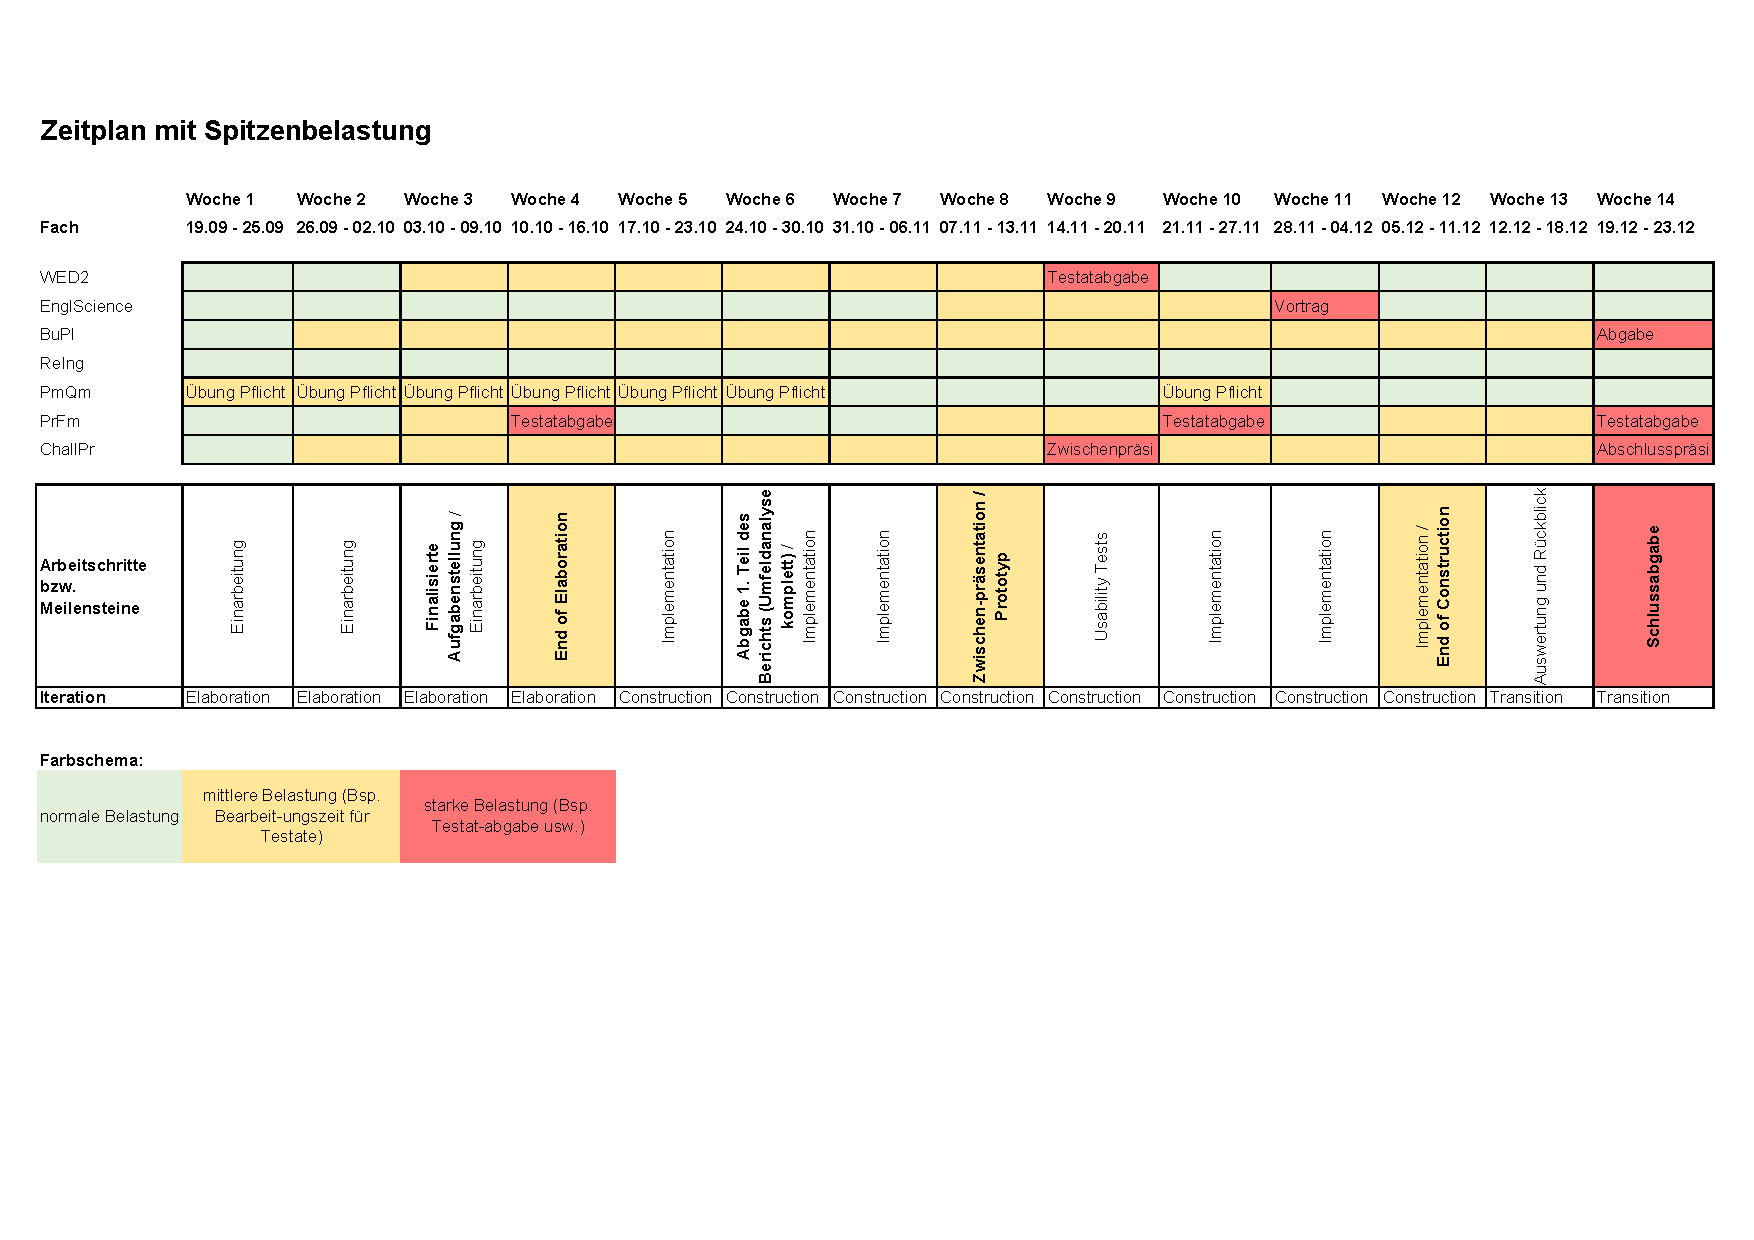
\includepdf[landscape=true]{PDFs/Zeitplan_Spitzenbelastung.pdf}
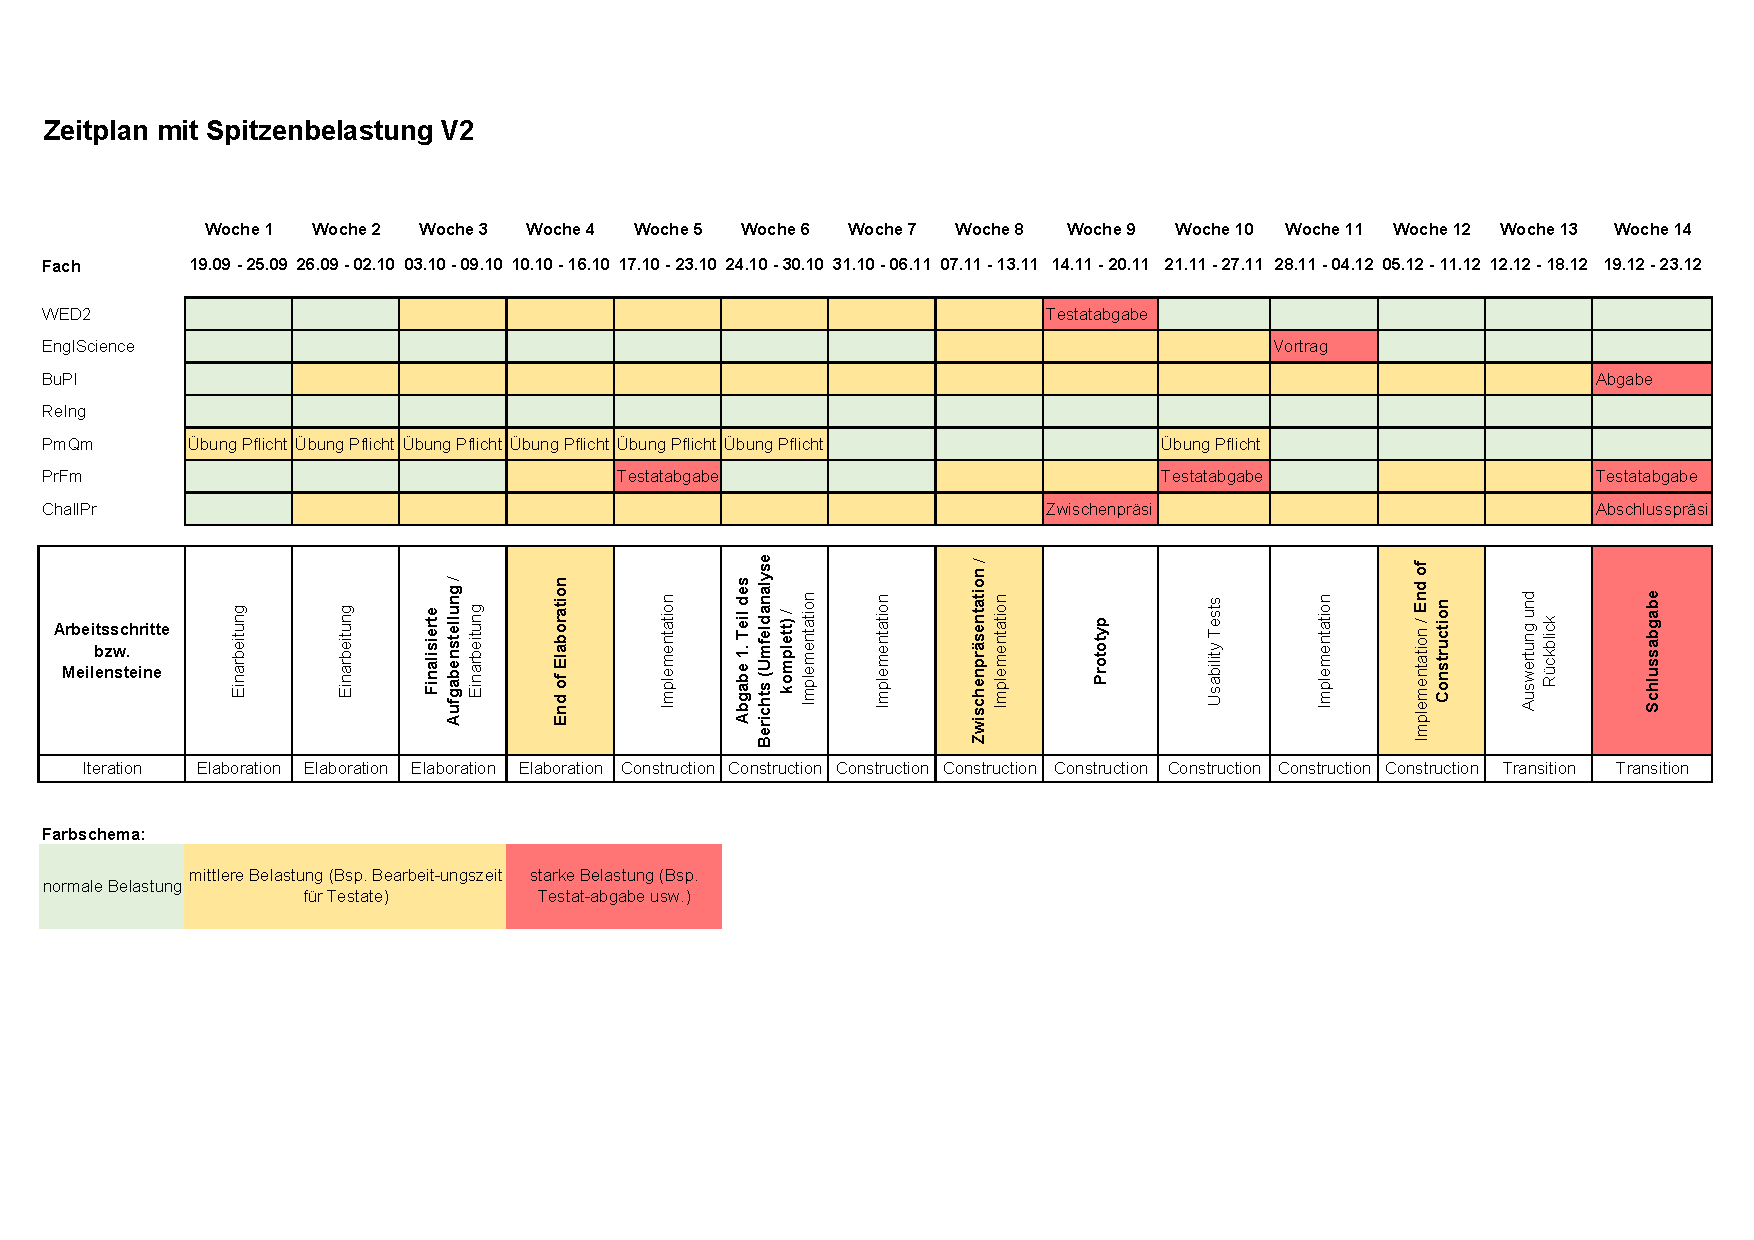
\includepdf[landscape=true]{PDFs/Zeitplan_SpitzenbelastungV2.pdf}
 
 \subsubsection{Rückblick zeitliche Planung}
 Rückblickend gesehen muss gesagt werden, dass der erste grob aufgestellte Zeitplan bei weitem nicht eingehalten werden konnte. Es wurde nicht damit gerechnet, dass die Ausarbeitung der Konzepte einen so grossen Teil der Zeit in Anspruch nehmen würde. Da sich die Konzeptausarbeitungen zu beginn der Arbeit befanden, verschoben sich durch den Mehraufwand alle dahinter gesetzten Termine. Auf der nächsten Seite ist der Zeitplan ersichtlich mit den effektiv Durchgeführten Arbeiten und Iterationen eingezeichnet. Zudem wurden auch die Belastungen der anderen Fächer gemäss der tatsächlichen Belastung aktualisiert.
 
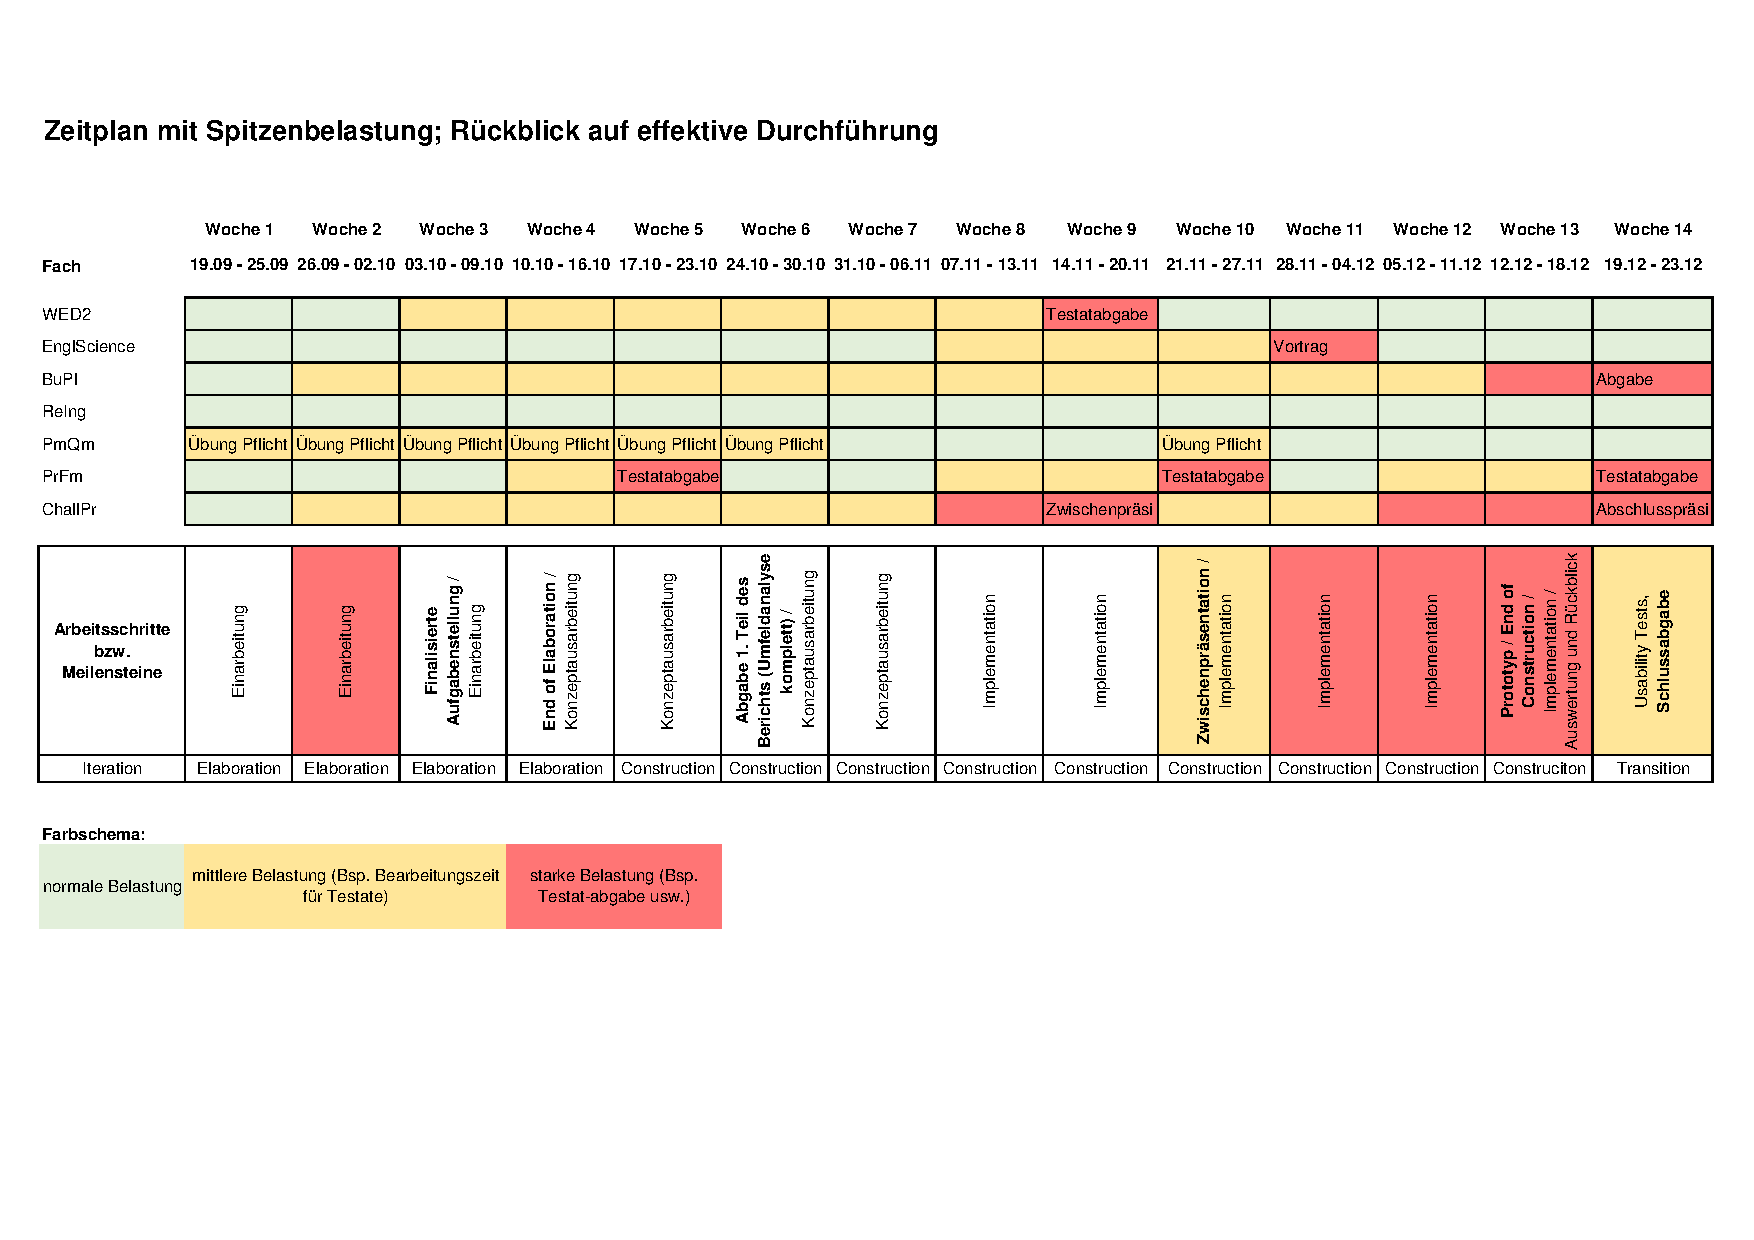
\includepdf[landscape=true]{PDFs/Zeitplan_SpitzenbelastungV3.pdf}
 
 \subsection{Meilensteine}
 %Die Meilensteine sollen konkret und messbar dargestellt werden.
 
 \begin{tabularx}{\linewidth}{|p{4.5cm}|c|c|X|}
 	\hline
 	\textbf{Meilenstein} & \textbf{Datum soll} & \textbf{Datum ist} &\textbf{Beschreibung} \\
 	\hline
 	Finalisierte Aufgabenstellung & 09.10.2016 & 09.10.2016 & Herr Heinzmann hat die zu erledigenden Arbeiten in einer Aufgabenstellung zusammengestellt und an die Studenten abgegeben. \\
 	\hline
 	End of Elaboration & 16.10.2016 & 16.10.2016 & Die Umfeldanalyse ist abgeschlossen und es ist bekannt, welche Arbeiten im Rahmen der Studienarbeit angegangen werden. \\
 	\hline
 	Erster Teil des Berichts komplett & 30.10.2016 & 25.10.2016 & Die Ergebnisse der Analyse-Phase sind vollständig niedergeschrieben, damit Herr Heinzmann diese gegenlesen kann. \\
 	\hline
 	Zwischenpräsentation & 13.11.2016 & 22.11.2016 & Die bisher erarbeiteten Ergebnisse wurden Herrn Heinzmann als Vortrag präsentiert. \\
 	\hline
 	Erster Prototyp & 13.11.2016 & 18.12.2016 & Die Code-Änderungen für eine verbesserte Usability wurden vollständig implementiert, damit in der Folgewoche die zweiten Usability-Tests durchgeführt werden können. \\
 	\hline
 	End of Construction & 11.12.2016 & 21.12.2016 & Alle Änderungen am Code wurden implementiert, sodass dieser wieder auf den cnlab-Server übertragen werden kann. \\
 	\hline
 	Schlussabgabe & 23.12.2016 & 23.12.2016 & Alle Dokumente wurden abgabekonform erstellt, die Dokumentation gebunden, der Code auf CD gebrannt und alles an Herrn Heinzmann abgegeben. \\
 	\hline
 \end{tabularx}
 
 
 
 \section{Zeiterfassung}
 Für alle Arbeiten werden in Redmine Arbeitspakete erfasst. Sofort nachdem ein Paket bearbeitet wurde, wird die Zeit darauf verbucht. Da alle Pakete einer Kategorie zugeordnet sind, kann am Ende des Projekts genau festgestellt werden, wie viel Zeit beispielsweise für alle Dokumentationen aufgewendet wurde.
 
 Die schlussendlich erfassten Pakete sind auf den folgenden Seiten abgebildet:
 
 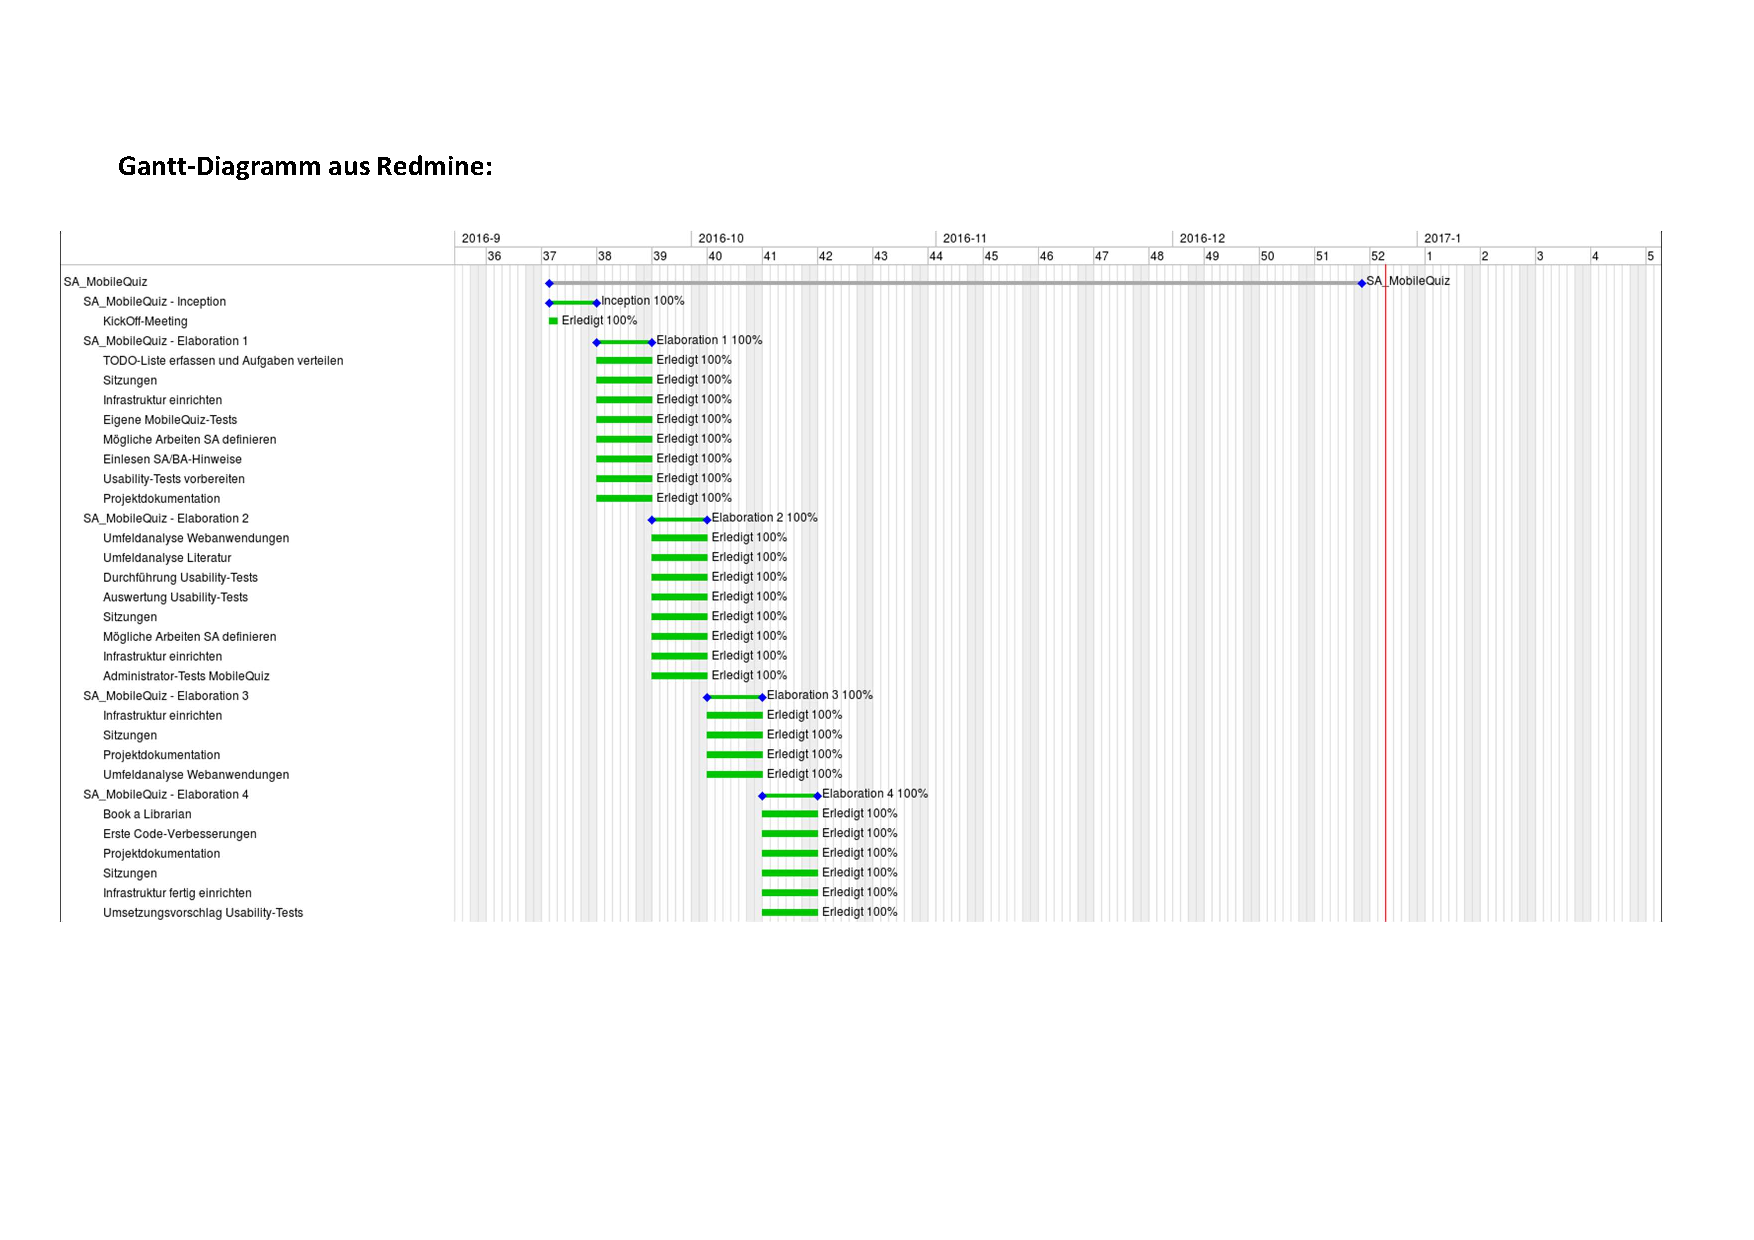
\includepdf[landscape=true,pages={1-3}]{PDFs/sa_mobilequiz-gantt_23-12-2016.pdf}
 
 \section{Auswertungen}
 \begin{figure}[H]
 	\centering
 	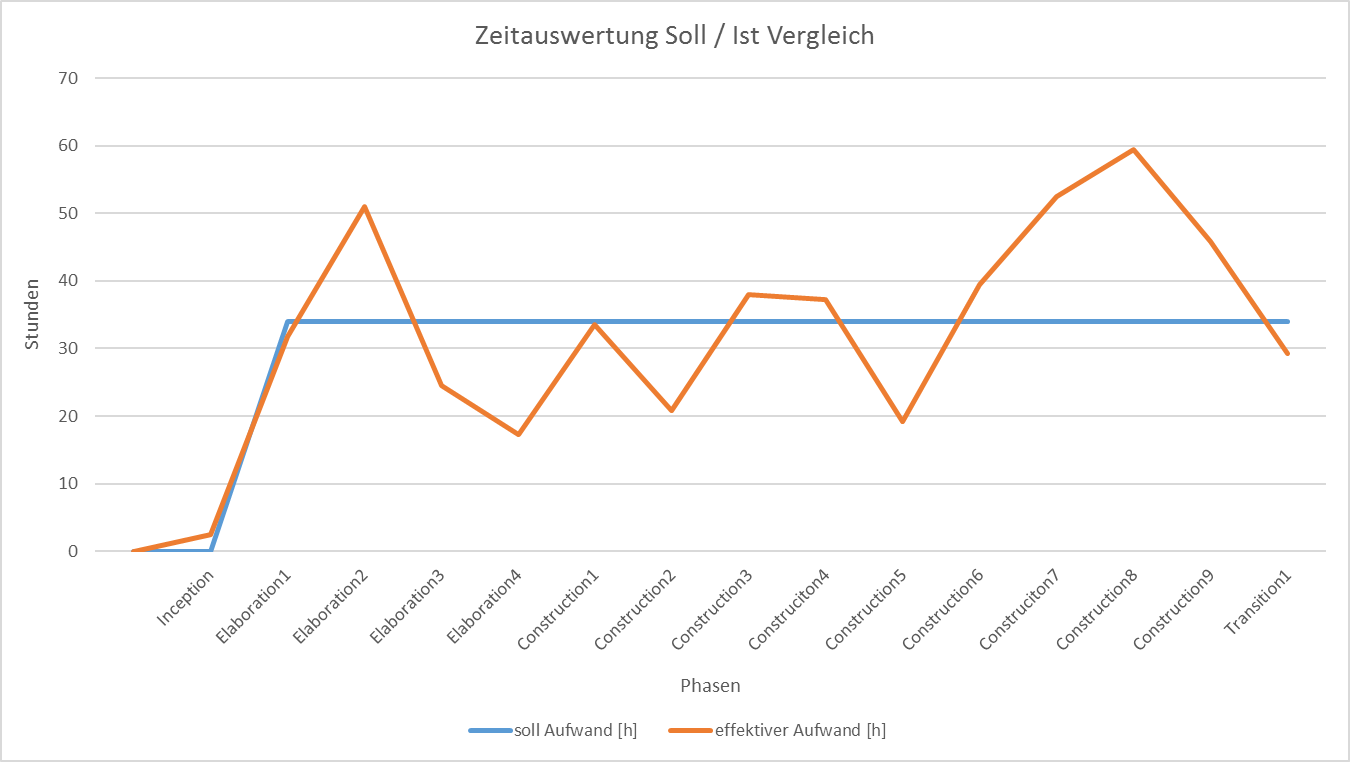
\includegraphics[width=1\textwidth]
 	{Images/ZeitauswertungSollIst.png}
 	\caption{Vergleich der Zeit Soll und Ist}
 \end{figure}
 
 Es wurden die Soll-Zeiten von 34 Stunden pro Woche den effektiv auf die Arbeitspakete gebuchten Zeiten gegenübergestellt. Die in der Mitte der Studienarbeit zu wenig geleisteten Stunden wurden gegen Ende der Studienarbeit mehr als eingeholt. Es wurden schlussendlich 502 Stunden geleistet.
 
 \bigskip
 
 Diese Stunden verteilen sich wie folgt auf die Ersteller dieser Arbeit:
 
 \begin{figure}[H]
 	\centering
 	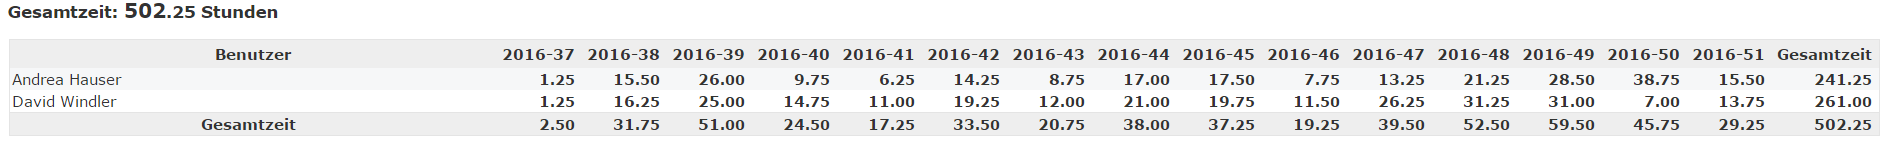
\includegraphics[width=1\textwidth]
 	{Images/ZeitauswertungBenutzer.png}
 	\caption{Zeitauswertung der geleisteten Zeit pro Person}
 \end{figure}
 
 Im Soll / Ist Vergleich der Zeitauswertung sieht man starke Schwankungen. Wenn man allerdings die Zeitauswertung aus kumulierter Sicht betrachtet, fallen diese Schwankungen nicht mehr so stark ins Gewicht. 
 
 \begin{figure}[H]
 	\centering
 	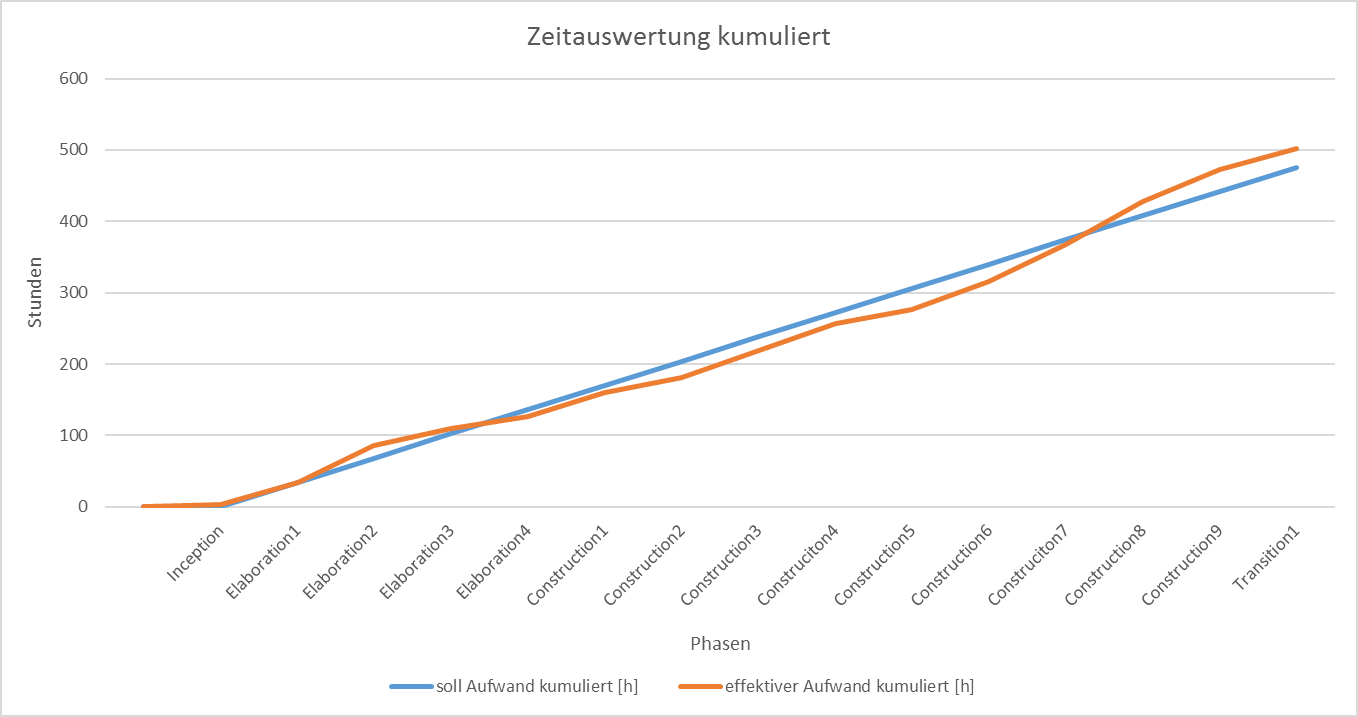
\includegraphics[width=1\textwidth]
 	{Images/ZeitauswertungKumuliert.png}
 	\caption{Zeitauswertung aus kumulierter Sicht}
 \end{figure}

Die unten stehende Grafik zeigt die Aufwände aufgeschlüsselt auf die einzelnen Kategorien.

\begin{figure}[H]
	\centering
	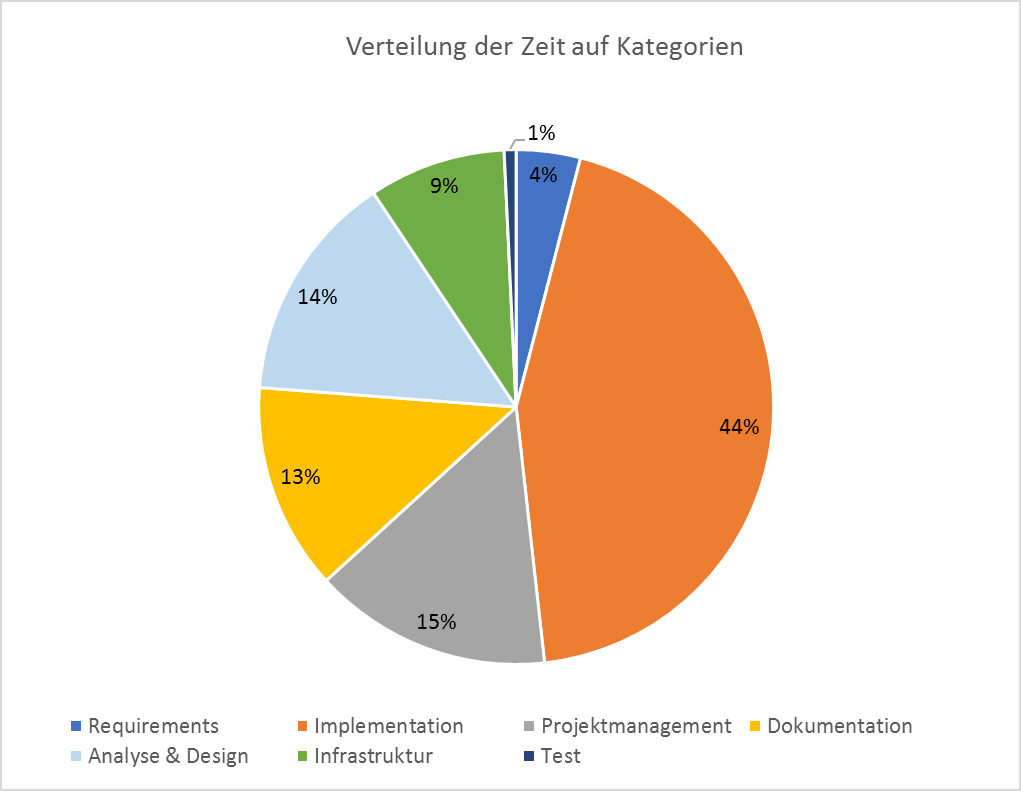
\includegraphics[width=0.8\textwidth]
	{Images/ZeitauswertungKategorien.png}
	\caption{Prozentuale Verteilung der Zeit auf die Kategorien}
\end{figure}
